\documentclass[11pt]{article}

\usepackage[margin=1in]{geometry}
\usepackage[T1]{fontenc}
\usepackage{lmodern}
\usepackage{microtype}
\usepackage{amsmath,amssymb,amsthm,mathtools}
\usepackage[dvipsnames]{xcolor}
\usepackage{tikz}
\usepackage{enumitem}
\usepackage[hidelinks]{hyperref}

\definecolor{courseblue}{HTML}{1F4E79}
\definecolor{lightblue}{HTML}{EAF2F8}
\definecolor{darkgray}{HTML}{333333}

\setlength{\parindent}{0pt}
\setlength{\parskip}{0.65em}
\setlist[itemize]{topsep=0.25em,itemsep=0.15em}

\theoremstyle{definition}
\newtheorem{definition}{Definition}
\newtheorem{example}{Example}
\theoremstyle{remark}
\newtheorem*{remark}{Remark}

\newcommand{\C}{\mathbb{C}}
\newcommand{\R}{\mathbb{R}}
\newcommand{\D}{\mathbb{D}}
\newcommand{\RePart}{\operatorname{Re}}
\newcommand{\ImPart}{\operatorname{Im}}

\begin{document}

\begin{center}
  \colorbox{lightblue}{%
    \begin{minipage}{0.94\textwidth}
      \vspace{0.55em}
      \begin{tabular*}{\textwidth}{@{\extracolsep{\fill}}lr}
        {\color{courseblue}\bfseries\LARGE Lecture 2} &
        {\color{courseblue}\bfseries\LARGE MATH 411}\\[0.35em]
        \textbf{Fall 2026} & \textbf{Date: Sep 4, 2026}\\
        & \textbf{Instructor: Manish Patnaik}
      \end{tabular*}
      \vspace{0.45em}
    \end{minipage}}
\end{center}

\section{The Extended Complex Plane}

Recall that every $z\in\C$ may be written in Cartesian or polar form:
\[
  z=a+ib=re^{i\theta},
  \qquad
  a=\RePart(z),\quad b=\ImPart(z),\quad r>0,\quad \theta\in\R.
\]
Its complex conjugate and modulus are
\[
  \overline z=a-ib,
  \qquad
  |z|=\sqrt{z\overline z}=\sqrt{a^2+b^2}.
\]

It is often useful to add one point, denoted by $\infty$, to the complex
plane.

\begin{definition}
The \emph{extended complex plane} is
\[
  \widehat{\C}=\C\cup\{\infty\}.
\]
\end{definition}

For $a,b\in\C$, we use the conventions
\[
  a+\infty=\infty+a=\infty,
  \qquad
  b\cdot\infty=\infty\cdot b=\infty\quad (b\ne0),
\]
and
\[
  \frac{a}{0}=\infty\quad (a\ne0),
  \qquad
  \frac{b}{\infty}=0.
\]
Expressions such as $\infty-\infty$, $0\cdot\infty$, $\infty/\infty$, and
$0/0$ remain undefined.

\section{Stereographic Projection}

Let
\[
  S^2=\{(x_1,x_2,x_3)\in\R^3:x_1^2+x_2^2+x_3^2=1\}
\]
be the unit sphere, and let $N=(0,0,1)$ be its north pole.  For
$P\in S^2\setminus\{N\}$, draw the line through $N$ and $P$.  It intersects
the plane $x_3=0$ in a unique point $Q$.

\begin{center}
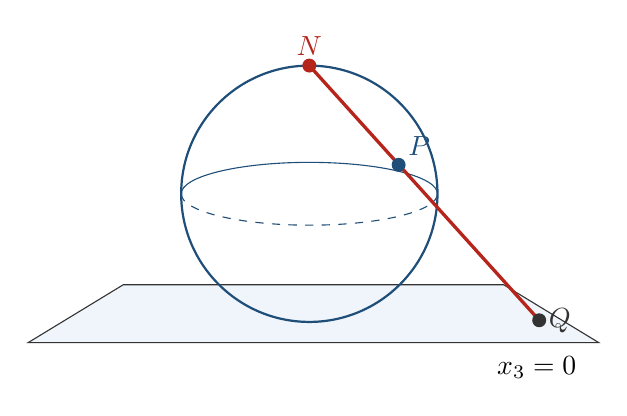
\begin{tikzpicture}[scale=1.05,>=stealth]
  \fill[lightblue,opacity=0.75]
    (-3.4,-0.25) -- (3.5,-0.25) -- (2.35,0.45) -- (-2.25,0.45) -- cycle;
  \draw[darkgray]
    (-3.4,-0.25) -- (3.5,-0.25) -- (2.35,0.45) -- (-2.25,0.45) -- cycle;
  \draw[courseblue,thick] (0,1.55) circle (1.55);
  \draw[courseblue,dashed] (-1.55,1.55) arc[start angle=180,end angle=360,
    x radius=1.55,y radius=0.38];
  \draw[courseblue] (1.55,1.55) arc[start angle=0,end angle=180,
    x radius=1.55,y radius=0.38];
  \coordinate (N) at (0,3.10);
  \coordinate (P) at (1.08,1.90);
  \coordinate (Q) at (2.78,0.02);
  \draw[very thick,BrickRed] (N) -- (Q);
  \fill[BrickRed] (N) circle (2.4pt) node[above] {$N$};
  \fill[courseblue] (P) circle (2.4pt) node[above right] {$P$};
  \fill[darkgray] (Q) circle (2.4pt) node[right] {$Q$};
  \node at (2.75,-0.55) {$x_3=0$};
\end{tikzpicture}
\end{center}

Identifying the $x_1x_2$-plane with $\C$, the point $Q$ corresponds to
\[
  \boxed{\displaystyle
    z=\frac{x_1+i x_2}{1-x_3}
  },
  \qquad P=(x_1,x_2,x_3).
\]

\begin{definition}
The map
\[
  \pi:S^2\setminus\{N\}\longrightarrow\C,
  \qquad
  P\longmapsto Q,
\]
is called \emph{stereographic projection}.
\end{definition}

The map $\pi$ is a bijection.  It extends to a bijection
\[
  \widehat\pi:S^2\longrightarrow\widehat\C
  \qquad\text{by setting}\qquad
  \widehat\pi(N)=\infty.
\]
Thus the extended complex plane may be viewed as a sphere.  Under
stereographic projection, circles on $S^2$ become circles or lines in
$\widehat\C$; circles through $N$ become lines in $\C$.

\begin{remark}
Substituting the equation of the line through $N$ and $P$ and imposing
$x_3=0$ verifies the displayed formula for $z$.
\end{remark}

\section{Functions of a Complex Variable}

Let $S\subseteq\C$.  A function of a complex variable is a map
\[
  f:S\longrightarrow\C,
  \qquad z\longmapsto w=f(z).
\]
Write
\[
  z=x+iy
  \qquad\text{and}\qquad
  w=u+iv.
\]
Then a complex-valued function can be expressed as
\[
  f(z)=u(x,y)+i\,v(x,y),
\]
where $u$ and $v$ are real-valued functions of the two real variables
$x$ and $y$.

\begin{example}[The squaring map]
For $f(z)=z^2$,
\[
  f(x+iy)=(x+iy)^2=(x^2-y^2)+i(2xy).
\]
Hence
\[
  u(x,y)=x^2-y^2,
  \qquad
  v(x,y)=2xy.
\]
Their first partial derivatives are
\[
  u_x=2x,\quad u_y=-2y,
  \qquad
  v_x=2y,\quad v_y=2x.
\]
\end{example}

\begin{example}[Complex conjugation]
For $f(z)=\overline z$,
\[
  f(x+iy)=x-iy,
  \qquad
  u(x,y)=x,\quad v(x,y)=-y.
\]
Thus
\[
  u_x=1,\quad u_y=0,
  \qquad
  v_x=0,\quad v_y=-1.
\]
\end{example}

\begin{example}[Power maps]
For $f(z)=z^n$, write $z=re^{i\theta}$.  Then
\[
  f(z)=r^n e^{in\theta}
      =r^n\cos(n\theta)+i\,r^n\sin(n\theta).
\]
Consequently,
\[
  u(r,\theta)=r^n\cos(n\theta),
  \qquad
  v(r,\theta)=r^n\sin(n\theta).
\]
The corresponding Cartesian formulas can be obtained by substituting
$r=\sqrt{x^2+y^2}$ and an argument $\theta$ of $x+iy$.
\end{example}

The relations
\[
  u_x=v_y,
  \qquad
  u_y=-v_x,
\]
are the \emph{Cauchy--Riemann equations}.  The squaring map satisfies them,
whereas complex conjugation does not.  We will study their significance
later.

\section{Visualizing Complex-Valued Functions}

The graph of a function $f:\C\to\C$ naturally lives in four real
dimensions, so it cannot be drawn in an ordinary three-dimensional plot.
Instead, we study how familiar subsets of the $z$-plane are transformed
into subsets of the $w$-plane.

For the squaring map $w=z^2$, consider the vertical line $x=x_0$.  Since
\[
  u=x_0^2-y^2,
  \qquad
  v=2x_0y,
\]
we may eliminate $y$ (when $x_0\ne0$) to obtain
\[
  u=x_0^2-\frac{v^2}{4x_0^2}.
\]
Thus vertical lines in the $z$-plane are mapped to parabolas in the
$w$-plane.

\begin{center}
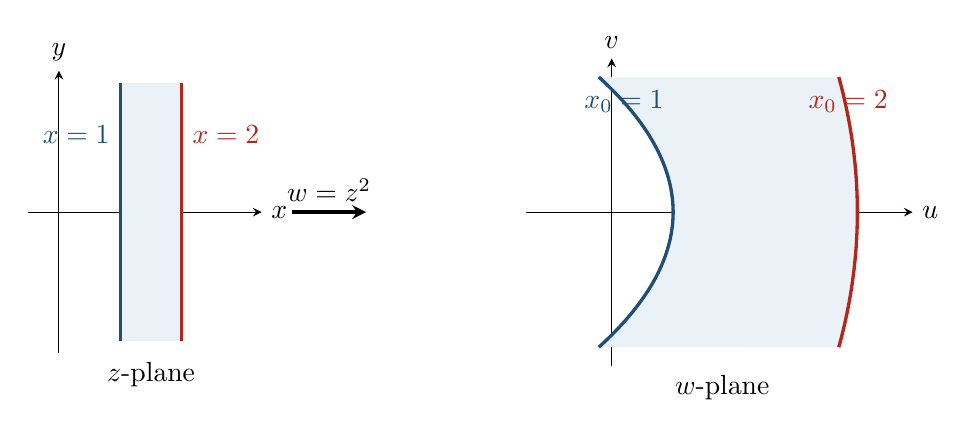
\begin{tikzpicture}[scale=0.78,>=stealth]
  \begin{scope}
    \draw[->] (-0.5,0) -- (3.3,0) node[right] {$x$};
    \draw[->] (0,-2.3) -- (0,2.3) node[above] {$y$};
    \fill[lightblue] (1,-2.1) rectangle (2,2.1);
    \draw[courseblue,very thick] (1,-2.1) -- (1,2.1)
      node[pos=0.8,left,courseblue] {$x=1$};
    \draw[BrickRed,very thick] (2,-2.1) -- (2,2.1)
      node[pos=0.8,right,BrickRed] {$x=2$};
    \node at (1.5,-2.65) {$z$-plane};
  \end{scope}

  \draw[->,very thick] (3.8,0) -- (5.0,0) node[midway,above] {$w=z^2$};

  \begin{scope}[xshift=9cm]
    \draw[->] (-1.4,0) -- (4.9,0) node[right] {$u$};
    \draw[->] (0,-2.5) -- (0,2.5) node[above] {$v$};
    \path[fill=lightblue]
      plot[domain=-2.2:2.2,samples=70] ({4-(\x*\x)/16},{\x})
      -- plot[domain=2.2:-2.2,samples=70] ({1-(\x*\x)/4},{\x})
      -- cycle;
    \draw[courseblue,very thick,domain=-2.2:2.2,samples=70]
      plot ({1-(\x*\x)/4},{\x});
    \draw[BrickRed,very thick,domain=-2.2:2.2,samples=70]
      plot ({4-(\x*\x)/16},{\x});
    \node[courseblue] at (0.2,1.8) {$x_0=1$};
    \node[BrickRed] at (3.85,1.8) {$x_0=2$};
    \node at (1.8,-2.85) {$w$-plane};
  \end{scope}
\end{tikzpicture}
\end{center}

In particular, for $x_0=1$ the image parabola is
\[
  u=1-\left(\frac v2\right)^2,
\]
while for $x_0=2$ it is
\[
  u=4-\left(\frac v4\right)^2.
\]
The strip $1<x<2$ maps to the region between these two parabolas.

\section{Basic Topology in the Complex Plane}

\begin{definition}
For $\alpha\in\C$ and $r>0$, the \emph{open disc} centered at $\alpha$ with
radius $r$ is
\[
  D(\alpha,r)=\{z\in\C:|z-\alpha|<r\}.
\]
The corresponding \emph{closed disc} is
\[
  \overline{D}(\alpha,r)=\{z\in\C:|z-\alpha|\le r\}.
\]
The open unit disc is denoted by
\[
  \D=D(0,1).
\]
\end{definition}

\begin{definition}
A subset $U\subseteq\C$ is \emph{open} if, for every $\alpha\in U$, there is
an $r>0$ such that
\[
  D(\alpha,r)\subseteq U.
\]
A subset $F\subseteq\C$ is \emph{closed} if its complement $\C\setminus F$
is open.
\end{definition}

\begin{definition}
Let $S\subseteq\C$ and $\alpha\in\C$.
\begin{itemize}
  \item The point $\alpha$ is an \emph{interior point} of $S$ if
    $D(\alpha,r)\subseteq S$ for some $r>0$.
  \item The point $\alpha$ is a \emph{boundary point} of $S$ if, for every
    $r>0$, the disc $D(\alpha,r)$ meets both $S$ and $\C\setminus S$.
  \item The point $\alpha$ is an \emph{adherent point} of $S$ if every disc
    $D(\alpha,r)$ meets $S$.
\end{itemize}
\end{definition}

Every interior point and every boundary point of $S$ is adherent to $S$.
Indeed, the set of adherent points is the closure of $S$, which is the union
of the interior of $S$ and its boundary.

\section{Limits}

\begin{definition}
Let $S\subseteq\C$, let $f:S\to\C$, and suppose $\alpha$ is adherent to
$S\setminus\{\alpha\}$.  We say that
\[
  \lim_{\substack{z\to\alpha\\ z\in S}} f(z)=w
\]
if, for every $\varepsilon>0$, there exists $\delta>0$ such that, for every
$z\in S$,
\[
  0<|z-\alpha|<\delta
  \quad\Longrightarrow\quad
  |f(z)-w|<\varepsilon.
\]
\end{definition}

This is the same $\varepsilon$--$\delta$ definition used for functions of a
real variable, with distance measured by the complex modulus.

\end{document}
